% center for academic English may have good resources
% font should 12pt -> 11pt
\documentclass[a4paper, twoside, 12pt]{report}

% Extra maths symbols (nexists)
\usepackage{amssymb}

%% Language and font encodings
\usepackage[english]{babel}
\usepackage[utf8]{inputenc}
\usepackage[T1]{fontenc}

%% Sets page size and margins
\usepackage[a4paper,top=3cm,bottom=2cm,left=3cm,right=3cm,marginparwidth=1.75cm]{geometry}

%% Useful packages
\usepackage{amsmath}
\usepackage{graphicx}
\usepackage[colorinlistoftodos]{todonotes}
\usepackage[colorlinks=true, allcolors=blue]{hyperref}

% Allow landscape
\usepackage{pdflscape}

% Controls spacing
\usepackage{parskip}

% For references
\usepackage[backend=biber]{biblatex}
\addbibresource{bibs/export.bib}




\title{Automatic Concept Extraction in a Video Classification Pipeline Using Natural Language Explanations}
\author{Roko Parac}
% Update supervisor and other title stuff in title/title.tex

\begin{document}
\begin{titlepage}

\newcommand{\HRule}{\rule{\linewidth}{0.5mm}} % Defines a new command for the horizontal lines, change thickness here

%----------------------------------------------------------------------------------------
%	LOGO SECTION
%----------------------------------------------------------------------------------------


\includegraphics[width=8cm]{title/logo.eps}\\[1cm] % Include a department/university logo - this will require the graphicx package
 
%----------------------------------------------------------------------------------------

\center % Center everything on the page

%----------------------------------------------------------------------------------------
%	HEADING SECTIONS
%----------------------------------------------------------------------------------------

\textsc{\LARGE MEng Individual Project}\\[1.5cm] % Name of your university/college
\textsc{\Large Imperial College London}\\[0.5cm] % Major heading such as course name
\textsc{\large Department of Computing}\\[0.5cm] % Minor heading such as course title

%----------------------------------------------------------------------------------------
%	TITLE SECTION
%----------------------------------------------------------------------------------------
\makeatletter
\HRule \\[0.4cm]
{ \huge \bfseries \@title}\\[0.4cm] % Title of your document
\HRule \\[1.5cm]
 
%----------------------------------------------------------------------------------------
%	AUTHOR SECTION
%----------------------------------------------------------------------------------------

\begin{minipage}{0.4\textwidth}
\begin{flushleft} \large
\emph{Author:}\\
\@author % Your name
\end{flushleft}
\end{minipage}
~
\begin{minipage}{0.4\textwidth}
\begin{flushright} \large
\emph{Supervisors:} \\
Dr. Alessandra Russo 

Dr. Luke Dickens \\[1.2em] % Supervisor's Name
\emph{Second Marker:} \\
Dr. Robert Chatley % second marker's name
\end{flushright}
\end{minipage}\\[2cm]
\makeatother

% If you don't want a supervisor, uncomment the two lines below and remove the section above
%\Large \emph{Author:}\\
%John \textsc{Smith}\\[3cm] % Your name

%----------------------------------------------------------------------------------------
%	DATE SECTION
%----------------------------------------------------------------------------------------

{\large \today}\\[2cm] % Date, change the \today to a set date if you want to be precise

\vfill % Fill the rest of the page with whitespace

\end{titlepage}

\begin{abstract}

The abstract will go here
\end{abstract}

\renewcommand{\abstractname}{Acknowledgements}
\begin{abstract}
The acknowledgements will go here
\end{abstract}

\tableofcontents
\listoffigures
\listoftables

\chapter{Introduction}

Natural language can be used as metadata for any sort of data.
To make it machine-readable and valuable for a task at hand, one needs to extract relevant pieces of information about it consistently.
If done successfully, given natural language explanations could even be used to explain unseen classification examples or improve the video classification performance.
In this project, a method for the automatic extraction of valuable information from language is studied as part of a bottleneck-based video classification pipeline.





\section{Problem Setup}

The project aims to design a general method for extracting valuable information from natural language.
The initial attempt at designing such a method intends to tackle a specific problem well before expanding its domain.
The problem this work is helping to solve is the problem of the classification of short baseball video sequences.
% TODO fix
In particular, it targets the MLB-V2E dataset  \cite{RefWorks:RefID:16-2021automatic}.
This dataset consists of the following:

 - A short video of a baseball sequence (\href{www.mlb.com}{MLB} (Major League Baseball) clips).
 
 - Label describing the outcome which occurred in it: strike, foul, ball, none, out.

 - Crowd-sourced brief explanation of why the outcome occurred.
 
 
\begin{center}
\begin{tabular}{ |p{1.5cm}|p{1.5cm}|p{9cm}|p{1.7cm}|  }
 \hline
 \multicolumn{4}{|c|}{Extract from MLB-V2E dataset} \\
 \hline
 id, $n$ & label, $l_n$ & explanation, $e_n$& video, $v_n$\\
 \hline
 1 & strike & The batter did not swing. The ball was in the strike zone. & N/A \\
 2 & foul & the batter hit the ball into the stands and it landed in foul territory & N/A \\
 3 & ball & The hitter didn’t swing. The ball was outside the strike zone. & N/A \\
 4 & none & The video did not load. & N/A \\
 5 & out & the batter hit the ball and it was caught by the fielder & N/A \\
 
 \hline
\end{tabular}
\end{center}


% TODO insert reference to the classifier %
Additionally, the problem is explored within the context of a concept bottleneck classifier. 
In that context, \textbf{concepts} are defined as syntactic generalisations of atomic sentences. 
Moreover, an \textbf{atomic sentence} is a sentence that an NLP expert cannot decompose into multiple sentences.
The system designed in this project should be general-purpose; changing the dataset on which the concept bottleneck classifier operates should immediately produce relevant concept sentences for a different dataset.

As such, this project aims to propose a novel method, combining techniques from natural language processing, deep learning and logic-based learning, that would extract domain-independent concept sentences.


\section{Limitations and Assumptions}
% Probably talk about in the initial project things.

At the moment, only the syntactic concept generalisation is being made. 
A consequence of using syntactic concept generalisation is that the events happening in the video are isolated as sentences with no content linking between them. 
Additionally, the tokens in a generalised concept sentence must first occur in the original one.
This procedure may result in grammatically incorrect sentences.
For example, consider a sentence: \emph{The left fielder caught the ball.}.
With our current approach, the system can extract the following sentence \emph{The fielder caught the ball.}.
However, the issue is that it can be unclear who \emph{the fielder} is now because it was previously determined by the adjective \emph{left}.

An extension might be able to relax this limitation.
The most straightforward possible approach for resolving this issue may replace \emph{the} with \emph{a} in a generalisation where additional information about the determined noun is removed.

More advanced generalisation could involve swapping words out for their synonyms.
An additional extension could involve linking entities from one sentence to another. 



\section{Objectives}

The objectives of this project are:

 - Develop and evaluate a general syntactic framework for extracting concept sentences from any given sentence. The process would be split into decomposing non-atomic sentences into atomic and generating concept sentences from atomic sentences.
 
 - Explore how does this framework aid deep neural network models in the context of video classification, namely whether an improvement is achieved for the MLB-V2E dataset \cite{RefWorks:RefID:16-2021automatic}.


 - Time permitting, generate a natural language explanation of the label chosen by the classifier. 


\section{Challenges}

This section highlights challenges that are anticipated to happen and a brief overview of its difficulties.
The section will be revised upon completion of the project once the topics' complexity is more evident.

The following questions will be difficult but necessary to answer as a part of this project:

 - \emph{How should a concept extracted from natural language be defined?} Making a helpful concept and immediately extensible to other domains may be difficult. One cannot use expert knowledge to help craft features that the subsequent architecture should use.
 
 
 - \emph{How will the concept extraction pipeline be scaled with a large amount of data?} The proposed system will include logic-based learning systems ILASP \cite{RefWorks:RefID:18-law2020ilasp} to extract syntactic concept sentences. 
 Unfortunately, the system is not scalable with respect to hypothesis space. On the other hand, more scalable alternative FastLAS \cite{RefWorks:RefID:19-law2020fastlas:} includes limitations that may be impossible to workaround.
 
 - \emph{How is an atomic sentence decomposed into a concept sentence?} This is the critical problem the system must resolve to be used.

 - \emph{How should the sentences be decomposed into atomic sentences?} This is one of the critical problems this system would need to resolve to be applied effectively. It may become a much more complex issue than concept sentence extraction, which can be designed as graph pruning of a dependency graph.
 


\section{Contributions}

Not relevant yet.

% What is the problem?
% Why is it interesting?
% What is the main idea for solving it?


\chapter{Background}

\section{Answer Set Programming}

Answer Set Programming  \cite{RefWorks:RefID:1-lifschitz2008answer} is a form of declarative programming, with a Prolog-like syntax suitable for solving NP-hard search problems.
However, it is based on a different computation mechanism than Prolog: stable model semantics \cite{RefWorks:RefID:21-fitting1992michael}.
Answer set solver is a program that generates stable models of an answer set program, which are solutions of an answer set program. 
The chosen answer set solver used throughout this project is clingo \cite{RefWorks:RefID:22-clingo}.

This section will briefly highlight the syntax of the answer set programs and the stable model semantics.

\subsection{Syntax}

Here are the types of rules in ASP\footnote{Disjunctive rules also exist, but they are omitted as they are not used in this work.}: 

 1. \emph{normal rule} -> $ h\; :- b_1, b_2, ..., b_n, not\; n_1, not\; n_2, ..., not\; n_o$
 
 2. \emph{hard constraint} -> $:- \; b_1, ..., b_n, not\; n_1, not\; n_2, ..., not\; n_o$
 
 3. \emph{choice rule} -> $lb\{h_1; ..., h_m\}ub\; :- \;  b_1, b_2, ..., b_n, not\; n_1, not\; n_2, ..., not\; n_o$
 
where $lb, ub$ are integers, $n_1,...,n_o$ are atoms and $b_1, ...,b_n$ are either atoms or aggregates.

Aggregates have the following syntax $lb\#agg\{e_1; ...; e_n\}ub$ where $lb, ub$ are ints, $agg$ is an aggregate function (e.g. $sum$) and $e_i$ is an aggregate element.
Additionally, aggregate element has the form  $t_1, ..., t_k : c_1, ..., c_j$ where $t_i$ is a term and $c_i$ is a literal.
 
This syntax is quite expressive. For instance, here are two ways to define a coin falling either on heads or tails.

\subsubsection{Method 1:}
\begin{verbatim}
coin(c1).
heads(C) :- coin(C), not tails(C).
tails(C) :- coin(C), not heads(C).
\end{verbatim}
\subsubsection{Method 2:}
\begin{verbatim}
coin(c1).
1 { heads(C); tails(C) } 1 :- coin(C).
\end{verbatim}

The results of these programs, i.e. the answer sets of the programs, are \{coin(c1), heads(c1)\} and \{coin(c1), tails(c1)\}.
It will be explained how they are computed in the subsequent subsection.

As seen in the example, a program can have multiple answer sets.
So, an additional piece of syntax is defined which evaluates whether some answer set is better than another.
This piece of syntax is referred to as a weak constraint.
It is of the form $:\sim {} b_1,..., b_n.[wt@lev, t1, ..., t_m]$
where $lev$ is an integer, $b_i$ a literal, and $t_i$ term.

\subsection{Semantics}

The Answer Set Programming is based on stable model semantics \cite{RefWorks:RefID:21-fitting1992michael}.

The answer set is defined as follows: 
\emph{Given a program P and a Herbrand interpretation X, X is an \textbf{answer set} of P iff X is a minimal Herbrand model of $RG(P)^X$ (reduct with respect to X).}

To understand the presented definition, one needs to know a few other concepts presented in this subsection.
Here the definitions for those concepts will mainly be explained intuitively rather than formally; for deeper understanding and more formal definitions, please refer to the \emph{Answer Set Programming} book \cite{RefWorks:RefID:23-lifschitz2019answer}. \\

\textbf{Herbrand interpretation} a program is an assignment of every element of the Herbrand base of that program to either true or false. \textbf{Herbrand base} of a program P is a set of all ground atoms that can be made using constants, predicate symbols, and functions of a program P.\\

When a Herbrand interpretation X satisfies all the rules in of a program, X is the \textbf{Herbrand model} of a program. X is also a minimal Herbrand model if there is no smaller subset X', also a Herbrand model.\\

\textbf{Relevant grounding} replaces variables with a program with constants available.
It iteratively fills up the rules by adding every rule whose elements of $body^+$(R) are heads of already included rules. 
The $body^+$ constraint ignores the $not$ atoms. 
For example, take P = \{p(X) :- q(X). q(a).\}. 
The first iteration of relevant grounding would create P' = \{q(a).\} while after the second one P' = \{q(a). p(a) :- q(a).\}\\

The \textbf{reduct of a program} P with respect to X ($P^X$) is a construct used to remove the $not\: c$ terms from a program.
Computing the reduct is done in the following manner. The solver assumes the X is a solution and iterates through every $not\: c$ within P. 
If $c$ is not in X (assumed to be false), then the $not\: c$ term is removed from the rule containing it. 
It essentially removes the need to worry about $not\: c$ since that term is satisfied.
On the other hand, if $c$ is in X, then the entire rule containing $not\: c$ is removed.
There is no need to consider the rule whose body is false since it cannot be satisfied.

Constructing the reduct of a \textbf{choice rule} has an additional step.
It is turned into either normal rules or a constraint.
Given a possible interpretation $X$, the choice rule $lb\{h_1; ..., h_m\}ub\; :- \;  b_1, b_2, ..., b_n, not\; n_1, ..., not\; n_o$ is converted in a following manner:

1. if $ lb \leq |\{h_1; ...; h_m\} \cap X| \leq ub$ then $h_i :- \;  b_1, b_2, ..., b_n, not\; n_1, ..., not\; n_o$ for is created for each $i \in \{1..m\}$

2. Otherwise, a constraint of the form $ :- \;  b_1, b_2, ..., b_n, not\; n_1, not\; n_2, ..., not\; n_o$ 
is created.\\

So, to check whether X is an answer set, one needs to compute a relevant grounding of a program. Then it needs to construct a reduct of that program with respect to X.
From the reduct, one can easily construct a minimal model M by starting from facts and iteratively adding heads of those rules with all body elements already in M.
Finally, if X = M, then X is an answer set.
Note that the head of a \textbf{constraint} is considered to be $\bot$. 
Hence, if the body of a constraint is satisfied, $\bot$ is added to M, so it cannot be equal to X.
In this manner, the constraints eliminate possible answer sets.






% Introduction to stable model semantics and its benefits over other forms of programming.
% Touch upon non-monotonicity. Its non-Turing completeness.

\section{Inductive Logic Programming}

% What is Inductive Logic Programming
Inductive Logic Programming \cite{RefWorks:RefID:42-muggleton1991inductive} is a field at an intersection of machine learning and logic programming.
In most cases, the goal of an inductive learning task is to learn a set of rules (a hypothesis H), which combined with the background knowledge B can entail every positive example while not entailing any negative example. 
Some systems use a weakened version of that statement to allow for noisy examples, such as the newer versions of ILASP \cite{RefWorks:RefID:55-law2018inductive}.

Many ILP systems have been developed over the years, such as Progol5 \cite{RefWorks:RefID:43-muggleton2000theory}, HAIL \cite{RefWorks:RefID:44-ray2003hybrid}, TopLog \cite{RefWorks:RefID:45-muggletontoplog:}, and TAL \cite{RefWorks:RefID:46-corapi2010inductive}.

The chosen system for this project is ILASP \cite{RefWorks:RefID:18-law2020ilasp}, a system that does the inductive learning of the answer sets programs.
Choosing a system that learns ASP is done because the ASP environment can effectively perform non-monotonic reasoning.\\

To understand the ILASP system fully, a few more definitions need to be introduced.

An atom A is \textbf{bravely entailed} if by a logic program P if it is included (true) in at least one answer set of P. 
On the other hand, an atom A is \textbf{cautiously entailed} if it is included (true) in all answer sets of P.

A pair $E = <E^{inc}, E^{exc}>$ (<inclusions, exclusions>) is a partial interpretation of sets of literals.
Answer set X extends E iff set of inclusions is a subset of X ($E^{inc} \subseteq X$) and X is disjoint with exclusions ($E^{exc} \cap A = \emptyset$).


The \textbf{language(inductive) bias} M, is a a pair $<M_h, M_b>$ which is used to construct the \textbf{search space} $S_M$ of a learning task.
The rule of the form  \\$ h \;{:-} b_1, b_2, ..., b_n, not\; n_1, not\; n_2, ..., not\; n_o$ is in $S_M$ iff:
 
 a) $h$ is compatible with $M_h$. This either means that $h$ is an atom compatible with $M_h$, an aggregate $lb\{h_1,.., h_m\}ub$ where each atom $h_i$ is compatible with $M_h$ or $h$ is empty.
 
 b) $b_i$ and $n_i$ are compatible with $M_b$.
 
 c) no variable does not appear in at least one element  of a positive body literal (the rule is safe). \\ 
 
Understanding what compatible refers to in the previous definition is the easiest through the means of an example.

\subsubsection{Inductive bias example}
\begin{verbatim}
#modeh(heads(var(coin))).
#modeh(tails(var(coin))).
#modeha(heads(var(coin))).
#modeha(tails(var(coin))).

#modeb(heads(var(coin))).
#modeb(tails(var(coin))).
#modeb(coin(var(coin))).
#modeb(coin(const(coin))).

#constant(coin, c1).
\end{verbatim}

The example above is a possible definition of the inductive bias for the simple coin problem written in ILASP-compatible syntax.
The \#modeh directive specifies that an atom can occur in the head of the rule. In this case, it defines that $heads(X)$ is compatible with $M_h$.
Similarly, the \#modeha defines that an atom can occur in the aggregate of the rule. Hence, it determines that  $lb\{..., heads(X), ...\}ub$ is a head compatible to $M_h$.
The \#modeb syntax defines that an atom can occur in the body either as a positive or negative atom.
Finally, the \#constant defines constants that can replace const functions.

Let $S_M$ be the search space constructed from the language bias M, B background knowledge, $E^+$/$E^-$ set of positive/negative examples, T = $<B, S_M, E^+, E^->$ is the \textbf{learning from answer set task} \cite{RefWorks:RefID:47-law2014inductive}.
The hypothesis H is a set of inductive solution iff:

1. It is a subset of search space $S_M$.

2. For every negative example $e^-$, there is no answer set A of the program $B \cap H$ which extends that example.

3. For every positive example $e^+$, there is an answer set A of the program $B \cap H$ which extends it.
\\

Notice that the positive examples are bravely entailed while the negative are cautiously entailed.\\

\subsubsection{Examples in ILASP}

\begin{verbatim}
#pos(
{heads(c1)},
{tails(c1)},
{coin(c1).}
).

#neg(
{tails(c2), heads(c2)},
{},
{coin(c2).}
).
\end{verbatim}

The shown piece of code is a simple definition of examples in ILASP. 
Both positive and negative take either 2 or 3 parameters. The first two are the set of inclusions $E^{inc}$ and the set of exclusions $E^{exc}$.
The third optional parameter is the context $C_e$ of an example.
The context of an example, $C_e$ is a set of rules and facts that are only relevant when explaining the example $e$.
With this parameter, the agent tries to find hypothesis H such that an answer set of $B \cap H \cap C_e$ extends $e$ (for positive $e$).
The analogue holds for negative examples. 
A formal definition of the Context-dependent Learning from Ordered Answer Sets framework can be found in work by Broda et al., \cite{RefWorks:RefID:56-broda2016iterative} which introduced context-dependent examples to ILASP. \\

FastLAS \cite{RefWorks:RefID:19-law2020fastlas:}, a much faster alternative to ILASP, has been developed recently.
Unfortunately, to get to the desired level of scale, the system operates with certain constraints which are too restrictive for this project.
For example, the programs constructed will generate at most one answer set.

% Link to Tutorials for FastLas, ILASP

\section{Natural Language Processing}

The critical requirement of this project is to extract syntactic concept sentences from the text corpus.
This section has a brief overview of the techniques applied to make the concept extraction possible.

The techniques presented in the following section are implemented by a popular library \emph{spacy} \cite{RefWorks:RefID:24-spacy} which has been utilised in this project. 
The language model currently used throughout the project is \emph{en\_wb\_gl\_lg}, but a more performant option may replace it after further investigation.

\subsection{Preprocessing Techniques}

\textbf{Tokenisation} separates the given text into smaller units named \emph{tokens}. 
It is common to split English text into words as tokens, as they carry meaning and are easy to extract.
The \emph{spacy} library implements such behaviour with it additionally separating punctuation into separate tokens.\\

\textbf{Sentence splitting} is a similar problem as tokenisation. It splits a text corpus into sentences before they are processed individually. \\

% TODO think of better %
\textbf{Word Normalisation} replaces words with a consistent form which greatly simplifies recognition of identical words.
Some of the reasons different forms of words arise are capitalisation (Cat, cat -> cat), acronyms (U.S.A/USA/U S A -> USA) and spelling variants (chequebook/cheque book -> cheque book). 
Most of the words can be modified by applying rule-based modifications, but there needs to be special handling of some words which have double meaning such as \emph{Turkey} (bird/country). \\


% tag spacy PoS 
\textbf{Part-of-speech tagging} attempts to determine which tag does a word have in the sentence.
The problem is much more complicated than the ones previously described as the part of speech can often be dependent on the meaning of the word in a sentence.
For example, the sentence \emph{I play the main character in a play} highlights how word \emph{play} can have two identically written words that can have different meanings and parts of speech.
The first occurrence of \emph{play} is a verb, and the second is a \emph{noun}.

The spacy library uses neural networks and statistical models to determine which tokens the library should assign which POS tag \cite{RefWorks:RefID:25-spacy}.
The classifier which spacy uses has a very high accuracy for the English language, with accuracy between 97-98\% depending on the model \cite{RefWorks:RefID:26-spacy}.


% http://nlpprogress.com/english/dependency_parsing.html - tracks state of the art

\subsection{Parsing}

\subsubsection{Dependency Parsing}

Dependency Parsing is a form of parsing that attempts to determine words' dependency within a sentence \cite{RefWorks:RefID:28-jurafsky2014speech}.

The resulting structure obtained is a dependency parse tree.
An example of a dependency parse tree can be seen in \ref{dependency-graph}.
This structure enables determining which purpose does a word serve in a sentence.
To illustrate why determining what purpose a word serves in a sentence may be helpful, here is a predicate/subject refresher:
\emph{The subject is a person/object who/what the sentence is about, while the predicate tells what the subject is or what it is doing} \cite{RefWorks:RefID:27-subject}.
From this definition, it is clear that one can easily extract an actor in a sentence if they know what it is doing.
The dependencies produced by the \emph{spacy} dependency parser are more precise as they follow \hyperlink{https://univesaldependencies.org}{Universal Dependencies}.
For instance, those dependencies distinguish between nominal and clausal subjects.
Please refer to the \hyperlink{https://univesaldependencies.org}{Universal Dependencies} to see a complete list of the dependencies available if needed. 

% How does it work? Maybe describe Mniri et al approach if lacking content

% What is the performance.
To evaluate the performance of a dependency parser, one uses labelled attachment score (LAS) and unlabelled attachment score (UAS) accuracy \cite{RefWorks:RefID:28-jurafsky2014speech}.
The former validates how well a word is assigned to its head and whether a correct dependency relation is assigned.
The latter score checks whether the head is assigned correctly.
Spacy's dependency parsing system slightly trails behind the state of the art approaches at the moment, with its UAS and LAS being at 95.1\% and 93.7\%, respectively. 
Mniri et al. \cite{RefWorks:RefID:29-mrini2019rethinking} developed the current state of the art model, with UAS/LAS scores at 97.4\% and 96.3\%.

\begin{figure}[h]
\caption{Dependency graph of \emph{The fielder caught the ball.}}
\centering
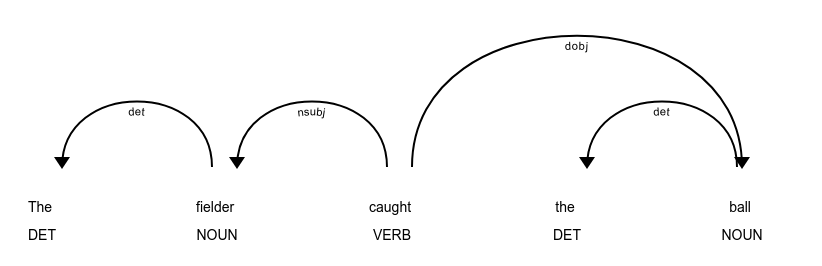
\includegraphics[width=\textwidth]{background/dependency_graph.png}
\label{dependency-graph}
\end{figure}

\subsubsection{Constituency Parsing}

Constituency Parsing is a form of syntactic parsing which assigns a structure to a sentence created by a context-free grammar \cite{RefWorks:RefID:28-jurafsky2014speech}.
This approach aims to group words into constituents, a group of words that behave as a single unit.
For example, one may group a sequence of words surrounding a noun into a noun phrase such as \emph{the Imperial students}.
Words grouped into constituents can be used as an intermediate form for semantic analysis and checking whether a sentence is grammatically correct.
In the context of this project, it will be utilised as a part of atomic sentence extraction.


The resulting structure produced by constituency parsing is a parse tree. 
An example of a tree parsed by a constituency parser can be seen in \ref{constituency-graph}.

\begin{figure}[h]
% https://parser.kitaev.io/
% INSERT https://spacy.io/universe/project/self-attentive-parser
% TODO find where labels are defined.
\caption{Parse tree of \emph{The fielder caught the ball.} as generated by spacy Berkley Neural Parser.}
\centering
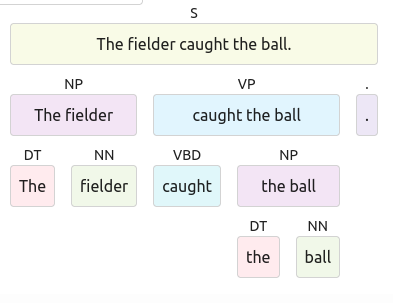
\includegraphics[width=0.8\textwidth]{background/constituency parse.png}
\label{constituency-graph}
\end{figure}

% How is it done if need more content?

% \section{Other Relevant Machine Learning Topics}
% 
% TODO
% 
% \subsection{Video Processing}
% 
% \subsubsection{Convolutional Neural Networks}
% 
% % Check those from their papers.
% 
% % Check more stuff from computer vision.
% 
% \subsubsection{Feature Extractors}
% 
% \subsection{Attention}






\chapter{Related Work}

\section{Inherited Work}
\label{inherited-work}

This thesis has not been started from scratch.

% TODO reference paper %
The project itself is a continuation of the \emph{Automatic Concept Extraction for Concept Bottleneck-based Video Classification} \cite{RefWorks:RefID:16-2021automatic} which my supervisors authored.
This paper is currently under review for the \href{https://iclr.cc/}{ICLR 2022} conference. \\

In this work, the following has been completed:

 Concept Discovery and Extraction Module (CoDEx) is proposed, which automatically uses video explanations to extract concepts.
 
 - Model has been evaluated to validate it obtains competitive performance with standard end-to-end models.
 
 - The concept-based architecture has been augmented with the attention mechanism, which enables verifying how important each concept is for a decision.
 
 - Two public datasets are constructed, MLB-V2E and MSR-V2E. Both combine crowd-sourced explanations with short video sequences. The difference is that the MSR-V2E focuses mainly on general videos while MLB-V2E is baseball-related.
\\

The CoDEx is a vital element of the project.
The presented Concept Discovery and Extraction Module in the paper consists of 6 stages: cleaning, extraction, grouping, completion, pruning, and vectorisation.
The cleaning stage removes videos/explanations which are corrupted.
The extraction step uses a constituency parser and a rule-based approach to determine whether a part of the sentence  should be included as a candidate concept. 
The rules are shown in the following table.

\begin{center}
\begin{tabular}{ |p{2cm}|p{12cm}|  }
 \hline
 \multicolumn{2}{|c|}{Rules determining whether a candidate concept should be included or excluded} \\
 \hline
 rule name & rule \\
 \hline
 Inclusion 1 & noun/pronoun → auxillary (optional) → particle (optional) → verb (optional) \\
 Inclusion 2 & noun/pronoun → auxiliary whose lemma is 'be' → any token \\
 Exclusion & subordinating conjunction \\
 
 \hline
 
\end{tabular}
\label{inclusion-exclusion-rules}
\end{center}

The completion stage looks up for concepts identified in some explanations while not other ones due to the behaviour of the constituency parser.
That stage is done by the substring lookup of existing concepts in all sentences where previous steps did not find that concept.

The grouping step attempts to group concepts with similar meanings using agglomerative clustering \cite{RefWorks:RefID:13-mullner2011modern}. 
It also removes concepts that have a small frequency.

The pruning stage attempts to keep highly informative concepts by picking the smallest concept subset such that the mutual information \cite{RefWorks:RefID:30-mackay2004information} between the label and a concept vector does not fall below a certain percentage $\gamma$.
This problem is not solved precisely, but rather concepts are inserted using a greedy approach until the mutual information between the label and the newly constructed vector is not below a percentage $\gamma$.


The vectorisation constructs the N x K concept matrix, where K is the number of concepts and N is the number of data points. 
The cell (n, k) is one if the concept k occurs for the data point n, zero otherwise.

\section{Video Classification}

Even though the work on video classification is not closely related to this thesis's contributions, it should serve as a performance benchmark of the entire system.

There are a few popular datasets for video classification out there, such as YouTube-8M \cite{RefWorks:RefID:10-abu-el-haija2016youtube-8m:} and Kinetics \cite{RefWorks:RefID:9-carreira2017quo}.
The YouTube-8M \cite{RefWorks:RefID:10-abu-el-haija2016youtube-8m:} is an extensive benchmark for general video classification with around 8 million clips and 4800 visual entities.
Mao et al. \cite{RefWorks:RefID:4-mao2019hierarchical} achieved very high performance on the YouTube-8M dataset using a deep convolutional graph neural network and a multi-level feature extractor.
Kinetics-700 \cite{RefWorks:RefID:14-carreira2019short} dataset is the latest version of the popular Kinetics dataset, which contains 700 human action classes and around 650000 video clips.
The top-performing model at the dataset has been designed by Yan et al. which uses Multiview Transformers for Video Recognition. 
The core idea of this approach is to input multiple different "views" of an input video into a transformer model to achieve better results.
This approach resulted in a model with an accuracy of 82.2\% on the Kinetics-700 dataset with the top-5 accuracy of 95.7\%.

YouTube-8M and Kinetics datasets are somewhat different to the dataset the majority of the project will address.
The MLB-V2E sequences look very similar, given that all of the sequences start with a pitcher throwing a ball.

A dataset much more closely related to our problem is the MLB-YouTube \cite{RefWorks:RefID:3-piergiovanni2018fine-grained} dataset.
The segmented video classification part of this dataset is the base for the MLB-V2E \cite{RefWorks:RefID:16-2021automatic} dataset which also includes crowd-sourced explanations. 
The MLB-YouTube dataset is quite different from the alternatives discussed in this section because the scene is very similar in all videos, only a single camera view is used, and the activity itself is only different because of the movement of one person.
The MLB-YouTube paper validates the InceptionV3 \cite{RefWorks:RefID:49-szegedy2016rethinking} and I3D \cite{RefWorks:RefID:9-carreira2017quo} networks performance on the constructed datasets shown in the table below.
These results should serve as a guide for the results of this project.

\begin{center}
\begin{tabular}{ |p{2cm}|p{1cm} p{1cm} p{1cm} p{1cm} p{1cm} p{1cm} p{1cm} p{1cm}|  }
 \hline
 \multicolumn{9}{|c|}{Per-class average precision for the multi-class baseball classification} \\
 \hline
 Method & Ball & Strike & Swing & Hit & Foul & In Play & Bunt & Hit by Pitch \\
 \hline
 Random & 21.8 & 28.6 & 37.4 & 20.9 & 11.4 & 10.3 & 1.1 & 4.5 \\
 InceptionV3 & 66.9 & 93.9 & 90.3 & 90.9 & 60.7 & 89.7 & 12.4 & 29.2 \\
 I3D & 62.5 & 91.3 & 88.5 & 86.5 & 47.3 & 75.9 & 16.2 & 21.0 \\
 \hline
 
\end{tabular}
\label{inclusion-exclusion-rules}
\end{center}


\section{Definition of Concept in Other Settings}

There are different angles to the definition of concepts in various works.
As mentioned, this project defines a concept as a syntactic generalisation of an atomic sentence.
However, this approach is not common in other works which do concept extraction.


Formal concept analysis \cite{RefWorks:RefID:31-ganter2012formal} is a method for knowledge representation based on the lattice theory which can be used to extract hierarchical concepts.
It defines two fundamental notions: a formal context and a formal concept. 
Formal context K := (G, M, I) consists of a set of objects G, set of attributes M and relation I on (G, M).
If (g, m) $\in$ I, object g has attribute m.
Using these attributes, set A$' $ is defined containing all attributes common to the objects in a set of objects A.
Additionally, set B$' $ contains objects that have all attributes in the set of relations B.
From these definitions, formal concept of context (G, M, I) is defined as a pair (A, B) such that A $\subseteq$ G, B $\subseteq$ M, B$' $ = A and A$' $ = B.

The Formal Concept Analysis with text analysis is mainly used to construct the concept hierarchy, where a concept refers to a phrase containing two words.

For example, work by Cimiano et al. \cite{RefWorks:RefID:32-cimiano2005learning} extracts verb/subject, verb/object/ and verb/prepositional phrase as candidate concepts.
Moreover, the Formal Concept Analysis is used by Anoop et al. \cite{RefWorks:RefID:33-anoop2019extracting} to extract concepts with their relationships from unstructured text.
The authors manually extract stemmed noun phrases as key phrases and use indications such as "is-a" to generate a formal context table.
This table is then used to extract hierarchical concepts.

On the other hand, TaxoLearn \cite{RefWorks:RefID:34-dietz2012taxolearn} by Dietz et al. does not use Formal Concept Analysis but also extracts noun phrases as concepts. The relevance of noun phrases is checked by computing how often they appear in a particular context compared to other contexts. It also uses a hierarchical clustering algorithm to construct a taxonomy.

Moreover, approaches such as the one by Koh et al. \cite{RefWorks:RefID:35-koh2020concept} define concepts as properties that the image may have. These properties need to be provided beforehand.

Finally, work such as the one by Fan et al. \cite{RefWorks:RefID:50-fan2004semantic} use expert defined terms, such as \emph{Lecture Presentation for Gastrointestinal Surgery}, as semantic concepts. 


\section{Concept-Based Explanations for Images and Text}

Concept-based explanations for images and text attempts is a more straightforward related problem.
Koh et al. \cite{RefWorks:RefID:35-koh2020concept} predict a set of pre-labelled concepts which they use to make a final classification.
The pipeline by Koh et al. is similar to the pipeline that will be used in this project, just that the concepts are automatically extracted instead of provided.
Yeh et al. \cite{RefWorks:RefID:36-yeh2019completeness-aware} propose a method that automatically extracts sets of pixels from an image that represent valuable concepts.
Similarly, Ghorbani et al. \cite{RefWorks:RefID:37-ghorbani2019automatic} propose another method that automatically extracts a set of visual concepts which are meaningful to humans.
All outlined methods are based on visual concept extraction, unlike this project's concept extraction, which will mainly focus on the events/actions in the baseball video sequence.


\section{Video Explanation}

Another related problem is that of Video Explanations. This project may even explore it at a later stage within the context of a concept extraction pipeline.

One famous dataset for video understanding is the MSR-VTT dataset \cite{RefWorks:RefID:40-jun2016msr-vtt:}. It is a large scale dataset with more than 10000 video clips in 257 popular categories of a video search engine.
Each video is annotated with roughly 20 sentences. 
A few different approaches for tackling this issue are presented as viable options in the paper, such as 2D Convolutions, 3D Convolutions, and RNNs.
One of the most performant methods on this dataset is CLIP2TV \cite{RefWorks:RefID:41-gao2021clip2tv:}, which utilises transformer-based techniques for both video and text representation.


The authors of the MLB-V2E \cite{RefWorks:RefID:16-2021automatic} have also constructed the MSR-V2E \cite{RefWorks:RefID:16-2021automatic} dataset, which uses the clips made available by the MSR-VTT and provides new classification labels and explanations.
This dataset will likely be used for the evaluation of this project.

\section{Semantic Concept Video Classification}

Semantic Concept Video Classification attempts to predict a set of predefined concepts from a video.
Predicting a set of predefined concepts from a video is closely related to a part of the pipeline in this project, which indicates which extracted concepts occur before predicting the outcome. 

The work by Fan et al. \cite{RefWorks:RefID:50-fan2004semantic} tries to predict semantically defined concepts by medical experts.
The paper proposes using salient objects, which are visually-distinguishable video components that human semantics understands, to model these semantical concepts.
Examples of notions salient objects attempt to represent are a face, voice, or a lecture slide.
Despite its benefits, the semantics of salient objects is quite simple, and it does not model relationships that happen over multiple frames in a video.
Newer work by Fan et al. \cite{RefWorks:RefID:51-jianping2007incorporating} also incorporates the possibility of a hierarchical concept classification. The approach also predicts atomic video concepts before constructing the higher-level ones and existing concept ontology.

Assari et al. \cite{RefWorks:RefID:52-assari2014video} represent a video by the co-occurrence of the semantic concepts before applying a classifier.
The concepts in this work are also predefined, but they represent a set of events rather than a set of objects.




\chapter{Project Plan*}

This section contains ideas on distributing work across the project, including the estimates for milestone completions.
Of course, estimating the complexity of an unknown problem is very challenging, so this section will also highlight which tasks may be omitted and include relevant extensions in case the actual project timeline allows for more/less work completed.\\

A portion of the work was completed before the interim report deadline. It is the following:

 - Concept generalisation dataset generation and cleaning. A few hundred concept generalisation examples were constructed using the available atomic sentences from the dataset. This dataset is also cleaned to remove incorrect atomic sentences.
 
 % TODO reference
 - Got familiar with the tools and techniques that will be used. In particular, I have greatly improved my knowledge of Answer Set Programming \cite{RefWorks:RefID:1-lifschitz2008answer}, spacy \cite{RefWorks:RefID:24-spacy} library and ILASP \cite{RefWorks:RefID:18-law2020ilasp} platform. The familiarisation also involved looking into other inductive logic programming frameworks like FastLAS \cite{RefWorks:RefID:19-law2020fastlas:}. 

 - Hand-crafted syntactic concept generalisation solution creation. The logic-based learning systems such as ILASP need an inductive bias used as a search space. So, creating a simple hand-crafted solution can help design the inductive bias for the system and serve as a benchmark of the performance of such a system. This work also involved the design of the knowledge representation.\\
 
 
The upcoming work has two major development milestones: completion of the syntactic concept generation and the atomic sentence generation.
Additionally, the 3rd large milestone would involve the generation of the explanations for the task.
The project may not reach this milestone depending on the success of the first two.
To accommodate the possibility that the milestones might be completed earlier than possible, two extensions are proposed: hierarchical concept extraction, concept linking across sentences and semantical concept extraction.
The hierarchical concept would involve creating a notion of a hierarchy between extracted concepts and utilising that information to make predictions.
On the other hand, concept linking across sentences would include a way to associate terms which occur in different sentences. For instance, in a pair of sentences \emph{Obama is a former US president. He finished his term in 2017.}, he could be linked to Obama.
Finally, the semantical concept extraction would involve extracting only relevant sentences for a given problem, such as a sentence \emph{The batter hit the ball} within the context of baseball.

\begin{landscape}

The current plan below involves general task descriptions, when they will be worked on and red lines indicating when the milestones will be completed. 
The following figure proposes a project plan and the tasks that will be attempted each week.

The project plan is shown in \ref{project-plan}. It gives rough estimates of dates when I plan to work on each specific project part.
This plan was designed with the following constraints in mind:

 - The research needs to be done early so that informed design decisions can be made.
 
 - It is expected that the atomic sentence generation is the most complex part of the project, followed by the concept generalisation implementation.
 
 - In the spring term, two week period allows for more work than the same period in the autumn term. 
 It is a consequence of taking three modules instead of four.
 Moreover, the summer term is completely available for project work, so two week period should be more productive than the same period in the spring term. Hence, the generation of atomic sentences has fewer regions shaded in than the concept generalisation despite being more complex.
 

\begin{figure}[h]
\caption{Project plan. Shaded areas represent times when I plan to be working on a specific part of the project.}
\centering
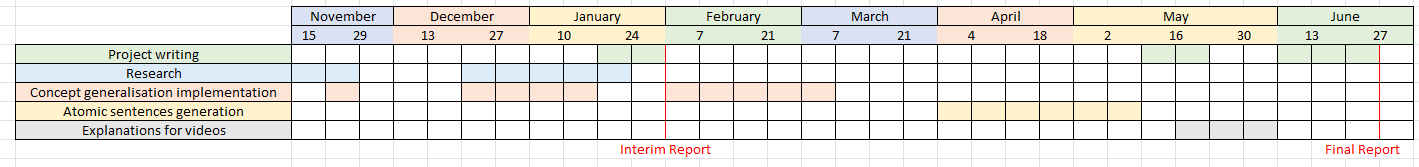
\includegraphics[width=1.6\textwidth]{project/project plan.PNG}
\label{project-plan}
\end{figure}


\end{landscape}
% Possible background additions:
% Positive/Negative examples ILASP.
% Semantic parsing maybe.

% Add a box plot somewhere


\chapter{Project Work}

This is temporary section until the project structure becomes more clear

\section{Learning to Extract Sentences}

Conditions that we wanted to achieve.

\subsection{Definitions}

There are two definitions that are used throughout the section:

% TODO add reference %
\textbf{Atomic Sentence:} A sentence is atomic if it cannot be decomposed in multiple simpler ones. Note that this equivalent to the definition used in logic.
However, the sentence structure considered in this project is often much more complex than the one considered in logics.


\textbf{Concept Sentence:} A syntactic generalisation of an atomic sentence, which satisfies the following 3 conditions:

 1. It is a valid sentence in its own right.
 
 2. True if the atomic sentence is.
 
 3. Obtained only through syntactic manipulation of an atomic sentence, a result of modifying the syntax tree of the sentence.
 
Concept sentences are often referred to as (syntactic) generalisations of a sentence in this report.



\textbf{Example number}: Splitting a given sentence into all its concepts sentences. 

Starting from the sentence: \\
\textit{The batter caught the ball in the air and sent it into the left field.} \\
we can extract the following atomic sentences: \\
\textit{The batter made contact with the ball in the air. The batter sent it into the left field.}
From these two sentences we can obtain four concept sentences: \\
\textit{The batter made contact with the ball in the air. The batter made contact with the ball. The batter sent it into the left field. The batter sent it into the field.}


The reason the project aims to extract all concept sentences from a particular sentence is two-fold:

 1. Concept sentences help associated differently worded explanations of the same concept.

 2. The final generated sentences are immediately usable for explanations.

\subsection{Problem Modelling}

% TODO: check if I am using generalisation

% INSERT reference
Inductive Logic Programming is approach is slightly different in the levels of commitment of knowledge representation than Deep Learning.
Deep Learning does not give any inductive bias to machine at all. 
The model must learn how to solve the problem from the data only.

Inductive Logic Programming uses a slightly weakened approach. 
We encode all the structure of the logic to learner which is encouraged to find all the possible theories within that structure and return the best one. 


% TODO: insert diagram for my overall pipeline.

\subsubsection{Preprocessing}

Before defining the logic structure that the learner should follow we need to learn how to encode the problem.

We are dealing with short text fragments which are first split into sentences.


% TODO: talk about the properties we would ideally like to achieve.
% Then mention usual stuff
% Then talk about ours.

Ideally we want to capture all the ways a human could explain that a particular event occurred.
In particular, we want the representation to satisfy the following:

1. Capture dependencies between words to determine whether a word is crucial to the meaning of a sentence.

2. Allow recognising slight word variations such as replacing words with its synonyms. It would be beneficial that words with same meaning are captured with a same representation.

3. Be compact. Smaller representations are quicker to process. 

4. Be domain independent. The framework itself should be translatable to different domains, so the representation should not contain domain-specific information.

5. Be interpretable. This is a requirement arising from a use of logic-based system.


% TODO: fix this section.
A common approach to encoding a word involves using concatenated dense-vector contextualised emdeddings of words. 
% INSERT references
Transformers, such as BERT, improve upon these embeddings by using self-attention mechanism to provide an even better representation for a sentence.
Dense-vector embeddings are useful because they are compact and tend to capture semantics of words (i.e. map similar words to similar value embeddings).

However, they are not interpretable making them unusable with our problem. 
But, our learning approach follows a similar idea of trying to capture the semantic relationships within a sentence.
We use dependency parse tree as a basis for both of our inductive logic learning tasks as it captures syntactic relationships between words.
Note that these are approximations of the semantic relationships between words.
In addition, words themselves are into the logical predicates.

Dependency tree gives rise to the following predicate:
\begin{verbatim}
    dep(l, token1, token2).
\end{verbatim}

It represents that there exists an arc from \textit{token1} to \textit{token2} with label \textit{l}.

Furthermore, it was noticed that in the examples for both concept and atomic sentence learning contained only the words used in the starting sentence.

As such, the problem which we are tacking could be modelled as whether or not we want to include the word in atomic/concept sentence.
These are denoted with predicates:
\begin{verbatim}
   in_generalised_sent(T). in_atomic_sent(T). 
\end{verbatim}
which represent that a token T is included in concept/atomic sentence given.

The possibility of multiple sentences arising from a given one is modelled with multiple answer sets. 



Unfortunately, this approach does not allow capturing slight word variations.
% TODO: write in which section it is described
However, these are handled at grouping stage which use the transfomer-based embeddings which have the necessary property. \\




% Consider making this as a diagram if it is too long.
\textbf{Example:} Converting a \emph{He threw a fast ball.} to a logical form and back.


1. Construct the dependency tree for a given sentence. For \emph{He threw a fast ball.} the dependency graph is shown at \ref{example-dependency-graph}.

2. Convert tokens in the tree to a logical form:

\begin{verbatim}
    token(tok0, "he").
    token(tok1, "threw").
    token(tok2, "a").
    token(tok3, "fast").
    token(tok4, "ball").
    token(tok5, ".").
\end{verbatim}

3. Convert arcs and root in a tree to predicates.
\begin{verbatim}
    root(tok1).
    dep(nsubj, tok1, tok0).
    dep(dobj, tok1, tok4).
    dep(punct, tok1, tok5).
    dep(det, tok4, tok2).
    dep(amod, tok4, tok3).
\end{verbatim}


\begin{figure}[h]
\caption{Dependency graph of \emph{He threw a fast ball.}}
\centering
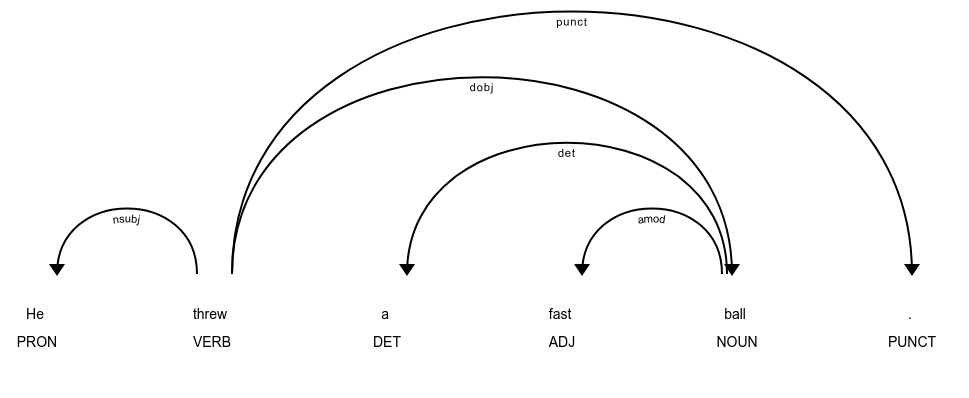
\includegraphics[width=\textwidth]{project-work/example_dependency_tree.png}
\label{example-dependency-graph}
\end{figure}

3. \textit{Clingo} is applied with atoms and predicates existing in: the background file, the learned solution file, and the generated logical form.

The resulting output is similar to:
\begin{verbatim}
Answer set #1:
{in_generalised_sent(tok0), in_generalised_sent(tok1), 
 in_generalised_sent(tok2), in_generalised_sent(tok3), 
 in_generalised_sent(tok4), in_generalised_sent(tok5)}.
    
Answer set #2:
{in_generalised_sent(tok0), in_generalised_sent(tok1), 
 in_generalised_sent(tok2), in_generalised_sent(tok4), 
 in_generalised_sent(tok5)}.
\end{verbatim}

4. For each answer set generated we reconstruct a sentence. 
The sentence reconstruction by converting each \textit{in\_generalised\_sent} token to the back to its string representation.
They are then joined by with spaces in the same order they originally appeared in.

For instance, for answer set \#2 we have tok0 -> "he", tok1 -> "threw", tok2-> "a", tok4 -> "ball", tok5 -> ".".
They are joined to a sentence \textit{he threw a ball .}

% TODO: reference truecasing
5. Post-processing clean-up involving truecasing and eliminating redundant spaces results in \emph{He threw a fast ball.} and \emph{He threw a ball.} \\



\subsubsection{Differences between atomisation and generalisation}

As noted in the previous section, atomisation and generalisation are handled in quite a similar manner.
In the current subsection, we will outline the difference between the two processes and why we have two processes in the first place.

Both are following the identical process as described in the example with only difference being in the background file and the learned solution.

Atomisation and generalisation approach generating multiple answer sets differently.
Generalisation learns the rule of the form: 
\begin{verbatim}
    in_generalised_sent(T) :- ...
    0 { in_generalised_sent(T) } 1 :- ...
\end{verbatim}
The latter rule results in two answer sets one of which contains the predicate in\_generalised\_sent, while the other one doesn't.

On the other hand, the atomisation task learns the rules of the following form:
\begin{verbatim}
    in_atomic_sent(T) :- ...
    splitting_tag(C).
\end{verbatim}
To produce multiple answer sets there are following additional rules in the background knowledge:
\begin{verbatim}
    candidate_start(T) :- splitting_tag(C), dep(C, T, _).
    candidate_start(T) :- splitting_tag(C), dep(C, _, T).
    0 { in_atomic_sent(T) : candidate_start(T) } 1.
\end{verbatim}
The idea for the latter approach is to start the atomisation from the tokens which should be in disjoint answer sets.
For example, in a sentence \emph{The ball is quick and accurate}, there is a \emph{conj} tag between \emph{quick} and \emph{accurate}.
With \emph{splitting\_tag(conj)} the learning process would be started with \emph{quick} and \emph{accurate} in different answer sets.
The rules with \emph{in\_atomic\_sent} as its head attempt to complete the sentence.
In the given example they learn to include \emph{The ball is}.
So, the overall task is to produces \emph{The ball is quick} and \emph{The ball is accurate} as final solutions.


Due to the more challenging nature of atomisation, the language bias of the learning tasks additionally includes more possible body predicates such as \emph{candiate\_start} and \emph{adjacent\_subj}.
The former is true for tokens which started the split while the latter recongises whether the sentence subject adjacent to currently included tokens.


\subsection{Example Encoding}

Generalisation and atomisation examples are given in the identical format.
Both consists of a given sentence followed by 1 to many sentences which are ways in which the provided sentence can be generalised/atomised.

Ideally, we want that the solution learned by ILASP produces possible solutions equal to the number of generalisations/atomisations.
% Equivalently, the number of answer sets produced for each sentence S be equal should be equal to the number of generalisations/atomisations of S.
% TODO: refer to background
ILASP allows defining two types of examples as outlined in \textit{section X}:


 - \#pos(ILASP)/$E^+$(definition), where $\forall<e, C> \in E^+$, $\exists A \in AS(B \cup C \cup H)$ such that $A$ extends $e$.
 
 - \#neg(ILASP)/$E^-$(definition), where $\forall<e, C> \in E^-$, $\nexists A \in AS(B \cup C \cup H)$ such that $A$ extends $e$.
 
Using these two constructs it is possible to define that we want exactly answer set for each possible generalisation/atomisation.
In particular, it is done by creating a positive example for each sentence that wish to produce. 
In addition, for each sentence example, a negative example is produced with \textit{goal} predicate in the exclusion, which defined in the context of the example. That predicate is true if in\_atomic\_sent/in\_generalised\_sent atoms are exactly corresponding to a positive example. \\


\textbf{Example}: Generating an ILASP-compatible examples for generalisation.

We will be encoding a premise sentence \textit{He threw a fast ball.} which can be generalised to: \textit{He threw a fast ball.} and \textit{He threw a ball.}

% TODO: insert reference.
1. Convert the premise sentence to logical form. This was shown in example X, so will not be shown again. 

2. For each possible generalisation, create a positive example. The context consists of predicates produced in 1) while the inclusion/exclusion appropriate in\_generalised\_sent tokens. For instance, \textit{He threw a ball.} would yield a following example:
\begin{verbatim}
#pos(example_id@noise_penalty,
{in_generalised_sent(tok0), in_generalised_sent(tok1), 
 in_generalised_sent(tok2), in_generalised_sent(tok4), 
 in_generalised_sent(tok5)},
{in_generalised_sent(tok3)}, % tok3 = "fast"
{
% all the predicates generated in 1)
}).
\end{verbatim}

3. Generate a negative example as follows:
\begin{verbatim}
#neg(example_id@noise_penalty,
{ },
{ goal },
{
% all the predicates generated in 1)

% He threw a fast ball.
goal :- in_generalised_sent(tok0), in_generalised_sent(tok1), 
        in_generalised_sent(tok2), in_generalised_sent(tok3), 
        in_generalised_sent(tok4), in_generalised_sent(tok5).
% He threw a ball.
goal :- in_generalised_sent(tok0), in_generalised_sent(tok1), 
        in_generalised_sent(tok2), in_generalised_sent(tok4), 
        in_generalised_sent(tok5)}, not in_generalised_sent(tok3).
}).
\end{verbatim}


\section{Managing Scalability Constraints}

% INSERT reference for this. %
A large challenge with logic based learning systems, such as ILASP, is a lack of scalability when dealing with large scale AI problems compared to other forms of machine learning.
The particular challenge that needed to be mitigated is the lack of scalability w.r.t size of the hypothesis space, which arises due to ILASP enumerating search space $S_M$ in full before finding a solution.
For example, consider the following simplified language bias definition:
\begin{verbatim}
#modeh(in_generalised_sent(var(token))).

#modeb(in_generalised_sent(var(token))).
#modeb(root(var(token))).
#modeb(dep(const(label), var(token), var(token))).

+ all the constant definitions.
\end{verbatim}

% Might be benficial to include a table how each rule reduced the search space size.

It took over 13 hours to generate a full search space on a machine with Intel Core i7 10510U 1.80GHz / 4.90GHz processor and 16 GiB of RAM.

% INSERT fastlas reference %
FastLAS is a system designed with alleviating this particular constraint but it is only able to deal with restricted version of learning tasks available in ILASP. 
Its inability to produce a solution with multiple answer set made it inapplicable for the current problem.
% TODO: insert reference to Mark's website
As such, the scalability issue was tackled using a meta-level definitions of the hypothesis space, which allow much greater flexibility compared to simple \textit{modeb}, \textit{modeh} statements. 
They allow constraining how rules are generated using ASP syntax.

Here are some examples of they are utilsed to restrict the search space presented in this section:
\begin{verbatim}
% Idea #1: Dep represents an arc in a tree. This allows 
% cutting out rules which are impossible to be satisfied.
    
% It is impossible to have more than 1 root per example.
:- #count{T : body(root(T))} > 1.

% Trees cannot have a relation to itself.
:- body(dep(_, X, X)).
:- body(naf(dep(_, X, X))).

% Trees are not reflexive
:- body(dep(_, X, Y)), body(dep(_, Y, X)).

% No depenency can go to the root
:- body(root(X)), body(dep(_, _, X)).

% Idea #2: Only allow two dep rules to occur in a body
% under certain conditions. 

% Pairs of dependency tags which can co-occur.
% Much smaller set of all possible pairs.
dep_chain(prep, pobj).
dep_chain(pobj, amod).
...

% Allow any rule with at most one dep predicate
allowed_dep_rule :- #count{L, V4, V5 : body(dep(L, V4, V5))} <= 1.
% Allow rule with two dep predicates if it is labels are white-listed
% as approved dep_chains and tokens are chained too.
allowed_dep_rule :- body(dep(L1, _, V2)), body(dep(L2, V2, _)), 
                    dep_chain(L1, L2), 
                    #count{L, V4, V5 : body(dep(L, V4, V5))} = 2.

:- not allowed_dep_rule.
\end{verbatim}

These kinds of modifications allowed the search space generation times to take less than a minute, starting from over 13 hours.


% Talk about memory when we actually fix it.
Probably need to talk a bit about memory if it is possible.


\section{Evaluation}

\subsection{Used Metrics}

Both atomisation and generalisation problems had an set of solutions of unknown size.
As such, an ideal metric would higher score if 2 sets are very similar compared to those that are far apart.

That would ideally involve a similarity in number of produced solutions and similarity of the elements themselves.

Due to this reason, a single number would have been hard to interpret since it would make it unclear what kinds of mistakes the model is making. 
For that reason, the evaluation is done with metrics which work with sets with possibly reduced notion of element equality.

The simplest metrics used were per-example Jaccard Index, precision and recall, with exact equality.
Jaccard Index is a metric with the following form:

 - $Jaccard(A, B) = \frac{card(A \cap B)}{card(A \cup B)}$ where $card$ represents set cardinatlity, $A$ a set containing true solutions, while $B$ contains predicated solutions.\\
 
Precision and recall are equivalent to the following for the problems in this thesis:
 
  - $Precision(A, B) = \frac{number \; of \; correctly \; predicted \; sentences}{number \; of \; predicated \; sentences} = \frac{card(A \cap B)}{card(B)}$
  
  - $Recall(A, B) = \frac{number \; of \; correctly \; predicted \; sentences}{number \; of \; correct \; sentences} = \frac{card(A \cap B)}{card(A)}$ \\
where  $card$ represents set cardinatlity, $A$ a set containing true solutions, while $B$ contains predicated solutions.

These metrics are also evaluated in a slightly relaxed manner using Levensthein distance.
$Jaccard\text{-}k$ is a notation used in this report where two elements of a set are equal if their Levensthein distance is less or equal $k$.
The same notational trick is used for $Recall\text{-}k$ and $Precision\text{-}k$.


% TODO: talk about consistency across runs for ILASP with cut-off 

% TODO: limitations
% - dependency parsing not perfect


% TODO: rename precision and recall with generalisation-precision/generalistaion-recall

% Probably doesn't justify a separate section. Most people do not have it.

% Need more explanation with designs for both generalisation and atomisation.
% Including limitations.

\chapter{Implementation}

In this section, the architecture of the entire concept bottleneck pipeline, as well as more detail unrelated to logical modelling, is presented.
Since, the work in this thesis is a continuation of the previous unpublished work, laid out in \autoref{inherited-work}, this section may include some parts which do not constitute my work. 
The * sign is used to signify the work that is not the work of the author of the thesis.


\section{Concept Bottleneck Pipeline*}

% TODO: fix X in picture, add boxes for the three parts, missing outlining X as attention module
\begin{figure}[h]
\caption{The full pipeline for the classification of MLB-V2E dataset using concept bottleneck model (adapted from \cite{RefWorks:RefID:16-2021automatic})}
\centering
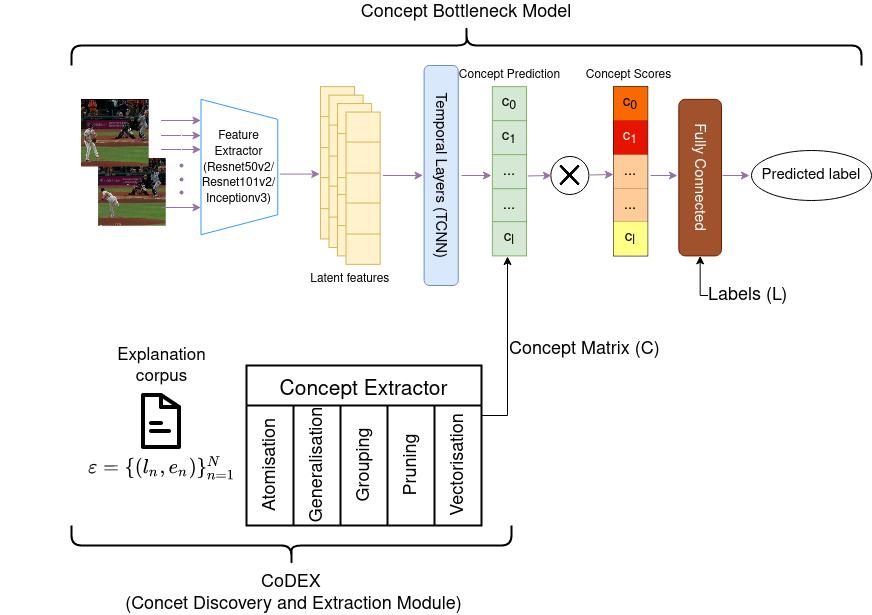
\includegraphics[width=\textwidth]{implementation/full architecture diagram.png}
\label{full-architecture-diagram}
\end{figure}

The concept bottleneck pipeline is shown in \ref{full-architecture-diagram}. 
Its purpose is to predict an output label correctly and in an interpretable manner.
The pipeline can be divided into concept extraction, concept prediction and label prediction pipeline. \\

\textbf{Concept Discovery and Extraction Pipeline (CoDEx)} is used to find an informative set of concepts for the problem at hand.
These concepts are extracted using human-generated explanations and labels in the dataset. 
The module consists of 5 parts: atomisation, generalisation, grouping, pruning, and vectorisation.

% INSERT chapter to reference.
The first two will be explained further in section X, while the latter 3 have been kept the same as explained in \autoref{inherited-work}. \\


\textbf{Concept Prediction Pipeline} has to predict the extracted concepts for the training images and varies depending on the problem type dealt with.
In all cases, it is a multi-label prediction model where output labels are probabilities that raw concepts occur.
The true labels for training are obtained from the concept matrix returned by the CoDEx module. \\

\textbf{Label Prediction Pipeline} has to predict the final output labels from the derived concepts. 
It consists of the attention mechanism, which highlights more relevant concepts for the prediction, and the fully connected layers. 
For further interpretability, the fully connected layer might be replaced with a neuro-symbolic component as a part of a future work.

\subsection{Dependencies}

\textbf{Sentence Transformers}: A library which provides access to pre-trained transformers. 
Since it is only used in the grouping stage, the ease of use of the library was the main reason for the selection of the library.


Finally, \textbf{numpy}, \textbf{scikit-learn}, \textbf{matplotlib}, \textbf{panadas} which all are famous Python libraries used with AI projects. \\

\chapter{Evaluation*}

% Luke feedback: Wee need to handle that more general concepts are often much more frequent then it is described 
% For example - bird has feathers should exist in all cases but it is only described when the feathers are special.

\chapter{Conclusion}

This paper demonstrates that a concept bottleneck model can be combined with human-generated explanations to improve NN explainability.
In doing so, we have discovered the following findings:
\begin{enumerate}
    \item \textbf{Logic-based methods can effectively be used to tackle some NLP seq2seq problems}.
    Such an approach was crucial as the datasets were tiny, consisting of only around 100 examples per problem.
    The dataset size made it impossible to use state-of-the-art NLP techniques such as transformers.
    On the other hand, the solutions made by hand-crafting or learning a set of rules could achieve good performance despite the dataset size.
    However, the limitation is the lack of scalability of the underlying ILASP \cite{RefWorks:RefID:54-ilasp} system used to learn a set of rules.
    It was applied successfully on the generalisation task, while it was far off its theoretical optimality guarantee for the atomisation task.
    When we applied it successfully, it did produce a better solution than a hand-crafted set of rules.
    
    
    \item \textbf{The newly proposed CoDEx pipeline significantly outperforms its predecessor}. 
    We have replaced the extraction part of the original pipeline with the new atomisation and generalisation stages.
    A new set of concepts is much more informable and better at predicting the final label.
    There is also an indication that the concepts it produced are better, but a large-scale human study must be conducted to validate such results.
    However, the CoDEx module still has room for improvement, as it cannot account for concepts occurring in the video but not explicitly in the explanation.
    This limitation leads to poor concept precision values.
    In addition, the limitation makes applying the sequential training procedure challenging, which splits the training of concept and label prediction parts of the network.
    Sequential training would be preferred, given that the joint training may not truly use concepts to predict the results.
    We further show that the CoDEx pipelines, although well performing, do not extract a valuable set of concepts given a set of general image descriptions.
    So, the applicability scope of this method needs to be further investigated. 
    But, we believe it should work for any domain where the human-generated explanation is written to describe the final label.
    
    \item \textbf{The proposed logic-based classification produces high-performing and easily explainable solutions}.
    We show that the method can be applied to the concept bottleneck pipeline exceptionally well.
    It helped achieve much better results for the MLB-V2E dataset \cite{RefWorks:RefID:16-2021automatic} compared to the original concept-bottleneck models while being completely interpretable.
\end{enumerate}

\section{Future work}

There are several directions possible to take this project further. We highlight some of the ideas for doing so in this section. \\

The most pressing concern is the CoDEx sparsity.
The human-generated explanations do not capture all of the concepts present in the concept matrix explicitly.
For example, both \emph{The ball was caught by the outfielder} and \emph{The outfielder got the pitch} would be extracted as separate concepts.
These sentences could have been grouped with some combination of hyper-parameters. 
However, finding such values often had an undesirable knock-on effect.
For example, \emph{The ball was outside of the strike zone} and \emph{The ball was inside of the strike zone} would almost always be grouped before the first two sentences are. \\
% INSERT An Inference Model for Semantic Entailment in Natural Language
To mitigate that issue, we might use models that solve the semantic entailment problem.
The semantic entailment task aims to determine whether some sentence S could be inferred by a sentence T.
Such information would allow us to group \emph{The ball was caught by the outfielder} and \emph{The outfielder caught the pitch} seamlessly.


Another possible direction could involve improving upon the video classification network.
We could enhance the current neural network architecture.
% INSERT Deep residual learning for image recognition
It consists of image features extracted by ResNet, from which motion features are captured using 1D convolution.
Much better architectures do exist, such as the ones discussed in \ref{video-classification}.
We expect that an improved architecture should improve concept prediction performance, which in turn improves the final class prediction.

Comparing the performance with the original concept bottleneck \cite{RefWorks:RefID:35-koh2020concept} would also be beneficial.
This work extends upon the original idea by mining the concepts from explanations.
% INSERT The caltech-ucsd birds-200-2011 dataset
The original work uses a human-engineered set of valuable concepts, which they applied to the CUB-birds dataset (X).
Comparing with the same dataset would give more insight into the generality of the concepts extracted by the CoDEx pipeline.


Moreover, the concept explanation quality should be evaluated using a human study, such as a Mechanical Turk analogous to \cite{RefWorks:RefID:16-2021automatic}.
Such a study would give more confidence regarding the quality of generated explanation.
In addition, we should also construct a human study interpreting the logic-based classification framework.

Finally, we could improve upon the atomisation procedure.
The atomisation procedure is the main culprit behind any concepts that are invalid sentences.
With the Jaccard score at around 0.5, the atomisation task has a lot of room for improvement. \\
% INSERT reference Exploring the limits of transfer learning with a unified text-to-text transformer.
A possible approach for handling this issue may involve trying to solve this problem using a seq2seq transformer such as T5.
It would require greatly extending the existing dataset, but it would undoubtedly perform better with a sufficient number of examples.

\chapter{Ethics}

The following section is based on the ethics checklist provided by the Computing Department. 
The checklist consists of a series of yes/no questions. 
If an answer was yes, there is an ethical issue that needs to be considered.
These answers will form a basis for the discussion in this chapter. \\


\emph{"Does the project involve human participants?"}
The project will involve human participants in two ways: 

    - For result validation. Some results obtained in the project will require an opinion of a participant, e.g. generated explanation correctness.
    
    - For dataset construction. The datasets used for this project, MLB-V2E \cite{RefWorks:RefID:16-2021automatic} and MSR-V2E \cite{RefWorks:RefID:16-2021automatic}, used human-generated explanations.

Both cases are not harmful to anyone involved. The only care that needs to be taken is regarding the personal information of the subjects involved, which is discussed in the following question.
Additionally, the participants involved in the dataset construction were compensated 15\$ per hour, as discussed in the paper under review \cite{RefWorks:RefID:16-2021automatic}.\\

\emph{"Does your project involve personal data collection and/or processing?"}

The dataset construction required subjects to explain a video in their own words.
But, this data is entirely anonymous and cannot be de-anonymised.
No explanation that is provided is in any way, shape or form personally identifiable information so that it can be linked back to a specific person.

Any data acquired from new participants during this project will be fully anonymised as well. \\

\emph{Will your project use or produce software for which there is a copyrighting licensing implication?}
The project uses three different, third-party pieces of software.
These are \emph{spacy} \cite{RefWorks:RefID:24-spacy}, \emph{ILASP} \cite{RefWorks:RefID:18-law2020ilasp}, and \emph{clingo} \cite{RefWorks:RefID:22-clingo}.
Both \emph{spacy} and \emph{clingo} use the MIT License \cite{RefWorks:RefID:53-mit}.
The MIT License is a permissive license that does not block any future publication and only requires the preservation of copyright and license notices.
On the other hand, \emph{ILASP} is free for use for university research, but it will require reaching out to Mark Law for commercial purposes \cite{RefWorks:RefID:54-ilasp}.
The licenses are not an issue as it stands. \\


To sum up, this project has no outstanding issues which need to be resolved.
\appendix
\chapter{Ethics}

The following section is based on the ethics checklist provided by the Computing Department. 
The checklist consists of a series of yes/no questions. 
If an answer was yes, there is an ethical issue that needs to be considered.
These answers will form a basis for the discussion in this chapter. \\


\emph{"Does the project involve human participants?"}
The project will involve human participants in two ways: 

    - For result validation. Some results obtained in the project have been obtained with human participants, e.g. generated explanation correctness.
    
    - For dataset construction. The datasets used for this project, MLB-V2E \cite{RefWorks:RefID:16-2021automatic} and MSR-V2E \cite{RefWorks:RefID:16-2021automatic}, used human-generated explanations.

Both cases are not harmful to anyone involved. The only care that needs to be taken is regarding the personal information of the subjects involved, which is discussed in the following question.
Additionally, the participants involved in the dataset construction were compensated 15\$ per hour, as discussed in the paper under review \cite{RefWorks:RefID:16-2021automatic}.\\

\emph{"Does your project involve personal data collection and/or processing?"}

The dataset construction required subjects to explain a video in their own words.
But, this data is entirely anonymous and cannot be de-anonymised.
No explanation that is provided is in any way, shape or form personally identifiable information so that it can be linked back to a specific person.

Any data acquired from new participants during this project will be fully anonymised as well. \\

\emph{Will your project use or produce software for which there is a copyrighting licensing implication?}
The project uses three different, third-party pieces of software.
These are \emph{spacy} \cite{RefWorks:RefID:24-spacy}, \emph{FastLAS} \cite{RefWorks:RefID:19-law2020fastlas:}, \emph{ILASP} \cite{RefWorks:RefID:18-law2020ilasp}, and \emph{clingo} \cite{RefWorks:RefID:22-clingo}.
\emph{FastLAS}, \emph{spacy} and \emph{clingo} use the MIT License \cite{RefWorks:RefID:53-mit}.
The MIT License is a permissive license that does not block any future publication and only requires the preservation of copyright and license notices.
On the other hand, \emph{ILASP} is free for use for university research, but it will require reaching out to Mark Law for commercial purposes \cite{RefWorks:RefID:54-ilasp}.
The licenses are not an issue as it stands. \\


To sum up, this project has no outstanding ethical issues which need to be resolved.

\chapter{Concept Bottleneck Model}
\label{concept-bottleneck-architectures}

This appendix presents networks used in Chapter \ref{concept-bottleneck-pipeline}.
In order to reproduce the results similar to this project, one needs to train them for 100 epochs, using the adam optimiser, and the batch size of 32. \\
The number next to layer name, such as \verb_5 Dense_, represents the number of outputs of that layer.
The network for the MLB-V2E dataset is shown in \ref{mlb-network-1} and \ref{mlb-network-2}, while the bird-flowers datset network is in \ref{birds-flowers-network}.

\begin{figure}[h]
\caption{MLB-V2E baseball network part 1}
\vspace{10pt}
\centering
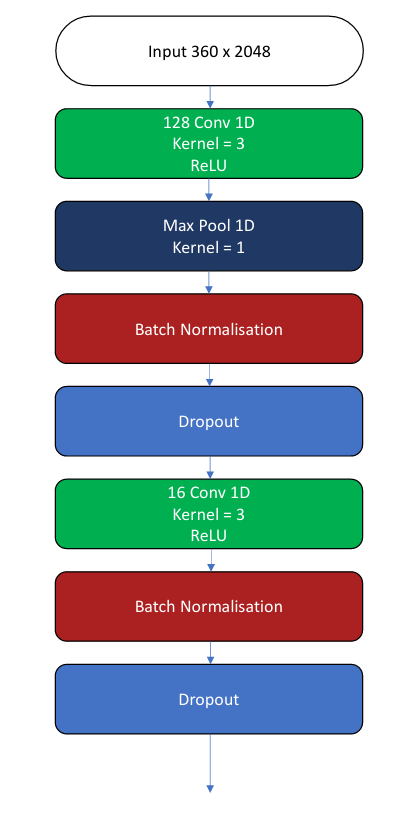
\includegraphics[width=0.6\textwidth]{appendix/mlb-network part 1.png}
\label{mlb-network-1}
\end{figure}

\begin{figure}[h]
\caption{MLB-V2E baseball network part 1}
\vspace{10pt}
\centering
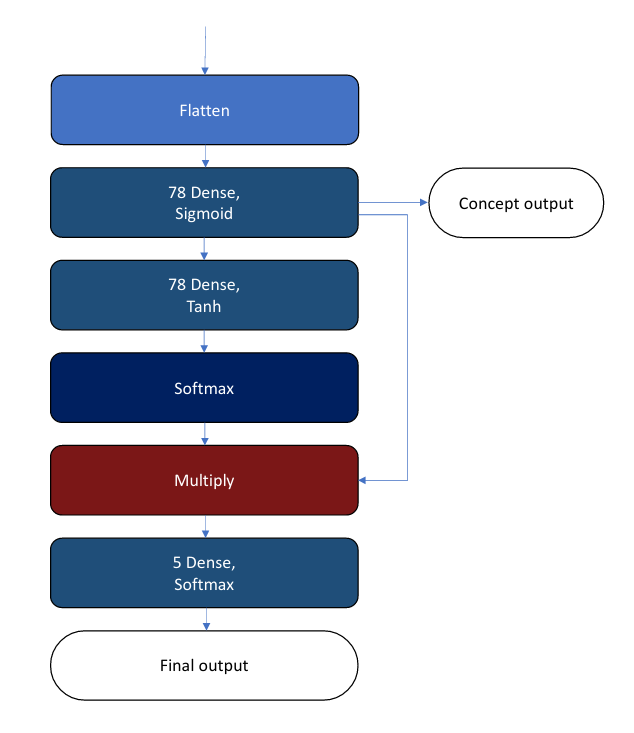
\includegraphics[width=\textwidth]{appendix/mlb network part 2.png}
\label{mlb-network-2}
\end{figure}

\begin{figure}[h]
\caption{MLB-V2E baseball network part 1}
\vspace{10pt}
\centering
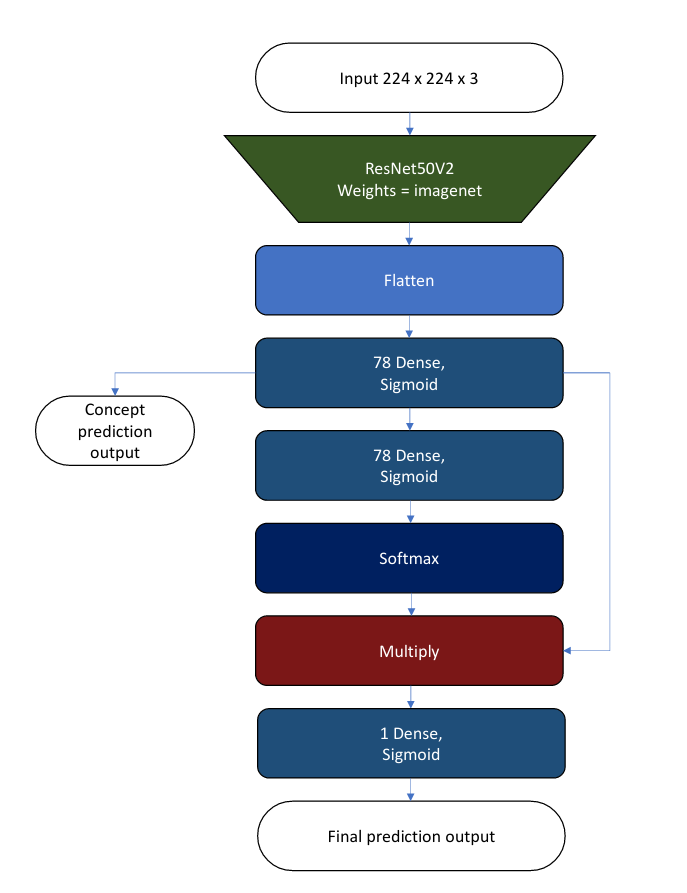
\includegraphics[width=\textwidth]{appendix/birds flowers prediction network.png}
\label{birds-flowers-network}
\end{figure}



%\bibliographystyle{alpha}
%\bibliography{bibs/sample}

%\bibliographystyle{plainnat}
%\bibliography{bibs/export.bib}

\printbibliography

\end{document}